
% Default to the notebook output style

    


% Inherit from the specified cell style.




    
\documentclass[11pt]{article}

    
    
    \usepackage[T1]{fontenc}
    % Nicer default font (+ math font) than Computer Modern for most use cases
    \usepackage{mathpazo}

    % Basic figure setup, for now with no caption control since it's done
    % automatically by Pandoc (which extracts ![](path) syntax from Markdown).
    \usepackage{graphicx}
    % We will generate all images so they have a width \maxwidth. This means
    % that they will get their normal width if they fit onto the page, but
    % are scaled down if they would overflow the margins.
    \makeatletter
    \def\maxwidth{\ifdim\Gin@nat@width>\linewidth\linewidth
    \else\Gin@nat@width\fi}
    \makeatother
    \let\Oldincludegraphics\includegraphics
    % Set max figure width to be 80% of text width, for now hardcoded.
    \renewcommand{\includegraphics}[1]{\Oldincludegraphics[width=.8\maxwidth]{#1}}
    % Ensure that by default, figures have no caption (until we provide a
    % proper Figure object with a Caption API and a way to capture that
    % in the conversion process - todo).
    \usepackage{caption}
    \DeclareCaptionLabelFormat{nolabel}{}
    \captionsetup{labelformat=nolabel}

    \usepackage{adjustbox} % Used to constrain images to a maximum size 
    \usepackage{xcolor} % Allow colors to be defined
    \usepackage{enumerate} % Needed for markdown enumerations to work
    \usepackage{geometry} % Used to adjust the document margins
    \usepackage{amsmath} % Equations
    \usepackage{amssymb} % Equations
    \usepackage{textcomp} % defines textquotesingle
    % Hack from http://tex.stackexchange.com/a/47451/13684:
    \AtBeginDocument{%
        \def\PYZsq{\textquotesingle}% Upright quotes in Pygmentized code
    }
    \usepackage{upquote} % Upright quotes for verbatim code
    \usepackage{eurosym} % defines \euro
    \usepackage[mathletters]{ucs} % Extended unicode (utf-8) support
    \usepackage[utf8x]{inputenc} % Allow utf-8 characters in the tex document
    \usepackage{fancyvrb} % verbatim replacement that allows latex
    \usepackage{grffile} % extends the file name processing of package graphics 
                         % to support a larger range 
    % The hyperref package gives us a pdf with properly built
    % internal navigation ('pdf bookmarks' for the table of contents,
    % internal cross-reference links, web links for URLs, etc.)
    \usepackage{hyperref}
    \usepackage{longtable} % longtable support required by pandoc >1.10
    \usepackage{booktabs}  % table support for pandoc > 1.12.2
    \usepackage[inline]{enumitem} % IRkernel/repr support (it uses the enumerate* environment)
    \usepackage[normalem]{ulem} % ulem is needed to support strikethroughs (\sout)
                                % normalem makes italics be italics, not underlines
    

    
    
    % Colors for the hyperref package
    \definecolor{urlcolor}{rgb}{0,.145,.698}
    \definecolor{linkcolor}{rgb}{.71,0.21,0.01}
    \definecolor{citecolor}{rgb}{.12,.54,.11}

    % ANSI colors
    \definecolor{ansi-black}{HTML}{3E424D}
    \definecolor{ansi-black-intense}{HTML}{282C36}
    \definecolor{ansi-red}{HTML}{E75C58}
    \definecolor{ansi-red-intense}{HTML}{B22B31}
    \definecolor{ansi-green}{HTML}{00A250}
    \definecolor{ansi-green-intense}{HTML}{007427}
    \definecolor{ansi-yellow}{HTML}{DDB62B}
    \definecolor{ansi-yellow-intense}{HTML}{B27D12}
    \definecolor{ansi-blue}{HTML}{208FFB}
    \definecolor{ansi-blue-intense}{HTML}{0065CA}
    \definecolor{ansi-magenta}{HTML}{D160C4}
    \definecolor{ansi-magenta-intense}{HTML}{A03196}
    \definecolor{ansi-cyan}{HTML}{60C6C8}
    \definecolor{ansi-cyan-intense}{HTML}{258F8F}
    \definecolor{ansi-white}{HTML}{C5C1B4}
    \definecolor{ansi-white-intense}{HTML}{A1A6B2}

    % commands and environments needed by pandoc snippets
    % extracted from the output of `pandoc -s`
    \providecommand{\tightlist}{%
      \setlength{\itemsep}{0pt}\setlength{\parskip}{0pt}}
    \DefineVerbatimEnvironment{Highlighting}{Verbatim}{commandchars=\\\{\}}
    % Add ',fontsize=\small' for more characters per line
    \newenvironment{Shaded}{}{}
    \newcommand{\KeywordTok}[1]{\textcolor[rgb]{0.00,0.44,0.13}{\textbf{{#1}}}}
    \newcommand{\DataTypeTok}[1]{\textcolor[rgb]{0.56,0.13,0.00}{{#1}}}
    \newcommand{\DecValTok}[1]{\textcolor[rgb]{0.25,0.63,0.44}{{#1}}}
    \newcommand{\BaseNTok}[1]{\textcolor[rgb]{0.25,0.63,0.44}{{#1}}}
    \newcommand{\FloatTok}[1]{\textcolor[rgb]{0.25,0.63,0.44}{{#1}}}
    \newcommand{\CharTok}[1]{\textcolor[rgb]{0.25,0.44,0.63}{{#1}}}
    \newcommand{\StringTok}[1]{\textcolor[rgb]{0.25,0.44,0.63}{{#1}}}
    \newcommand{\CommentTok}[1]{\textcolor[rgb]{0.38,0.63,0.69}{\textit{{#1}}}}
    \newcommand{\OtherTok}[1]{\textcolor[rgb]{0.00,0.44,0.13}{{#1}}}
    \newcommand{\AlertTok}[1]{\textcolor[rgb]{1.00,0.00,0.00}{\textbf{{#1}}}}
    \newcommand{\FunctionTok}[1]{\textcolor[rgb]{0.02,0.16,0.49}{{#1}}}
    \newcommand{\RegionMarkerTok}[1]{{#1}}
    \newcommand{\ErrorTok}[1]{\textcolor[rgb]{1.00,0.00,0.00}{\textbf{{#1}}}}
    \newcommand{\NormalTok}[1]{{#1}}
    
    % Additional commands for more recent versions of Pandoc
    \newcommand{\ConstantTok}[1]{\textcolor[rgb]{0.53,0.00,0.00}{{#1}}}
    \newcommand{\SpecialCharTok}[1]{\textcolor[rgb]{0.25,0.44,0.63}{{#1}}}
    \newcommand{\VerbatimStringTok}[1]{\textcolor[rgb]{0.25,0.44,0.63}{{#1}}}
    \newcommand{\SpecialStringTok}[1]{\textcolor[rgb]{0.73,0.40,0.53}{{#1}}}
    \newcommand{\ImportTok}[1]{{#1}}
    \newcommand{\DocumentationTok}[1]{\textcolor[rgb]{0.73,0.13,0.13}{\textit{{#1}}}}
    \newcommand{\AnnotationTok}[1]{\textcolor[rgb]{0.38,0.63,0.69}{\textbf{\textit{{#1}}}}}
    \newcommand{\CommentVarTok}[1]{\textcolor[rgb]{0.38,0.63,0.69}{\textbf{\textit{{#1}}}}}
    \newcommand{\VariableTok}[1]{\textcolor[rgb]{0.10,0.09,0.49}{{#1}}}
    \newcommand{\ControlFlowTok}[1]{\textcolor[rgb]{0.00,0.44,0.13}{\textbf{{#1}}}}
    \newcommand{\OperatorTok}[1]{\textcolor[rgb]{0.40,0.40,0.40}{{#1}}}
    \newcommand{\BuiltInTok}[1]{{#1}}
    \newcommand{\ExtensionTok}[1]{{#1}}
    \newcommand{\PreprocessorTok}[1]{\textcolor[rgb]{0.74,0.48,0.00}{{#1}}}
    \newcommand{\AttributeTok}[1]{\textcolor[rgb]{0.49,0.56,0.16}{{#1}}}
    \newcommand{\InformationTok}[1]{\textcolor[rgb]{0.38,0.63,0.69}{\textbf{\textit{{#1}}}}}
    \newcommand{\WarningTok}[1]{\textcolor[rgb]{0.38,0.63,0.69}{\textbf{\textit{{#1}}}}}
    
    
    % Define a nice break command that doesn't care if a line doesn't already
    % exist.
    \def\br{\hspace*{\fill} \\* }
    % Math Jax compatability definitions
    \def\gt{>}
    \def\lt{<}
    % Document parameters
    \title{ROC for Feature Detection}
    
    
    

    % Pygments definitions
    
\makeatletter
\def\PY@reset{\let\PY@it=\relax \let\PY@bf=\relax%
    \let\PY@ul=\relax \let\PY@tc=\relax%
    \let\PY@bc=\relax \let\PY@ff=\relax}
\def\PY@tok#1{\csname PY@tok@#1\endcsname}
\def\PY@toks#1+{\ifx\relax#1\empty\else%
    \PY@tok{#1}\expandafter\PY@toks\fi}
\def\PY@do#1{\PY@bc{\PY@tc{\PY@ul{%
    \PY@it{\PY@bf{\PY@ff{#1}}}}}}}
\def\PY#1#2{\PY@reset\PY@toks#1+\relax+\PY@do{#2}}

\expandafter\def\csname PY@tok@w\endcsname{\def\PY@tc##1{\textcolor[rgb]{0.73,0.73,0.73}{##1}}}
\expandafter\def\csname PY@tok@c\endcsname{\let\PY@it=\textit\def\PY@tc##1{\textcolor[rgb]{0.25,0.50,0.50}{##1}}}
\expandafter\def\csname PY@tok@cp\endcsname{\def\PY@tc##1{\textcolor[rgb]{0.74,0.48,0.00}{##1}}}
\expandafter\def\csname PY@tok@k\endcsname{\let\PY@bf=\textbf\def\PY@tc##1{\textcolor[rgb]{0.00,0.50,0.00}{##1}}}
\expandafter\def\csname PY@tok@kp\endcsname{\def\PY@tc##1{\textcolor[rgb]{0.00,0.50,0.00}{##1}}}
\expandafter\def\csname PY@tok@kt\endcsname{\def\PY@tc##1{\textcolor[rgb]{0.69,0.00,0.25}{##1}}}
\expandafter\def\csname PY@tok@o\endcsname{\def\PY@tc##1{\textcolor[rgb]{0.40,0.40,0.40}{##1}}}
\expandafter\def\csname PY@tok@ow\endcsname{\let\PY@bf=\textbf\def\PY@tc##1{\textcolor[rgb]{0.67,0.13,1.00}{##1}}}
\expandafter\def\csname PY@tok@nb\endcsname{\def\PY@tc##1{\textcolor[rgb]{0.00,0.50,0.00}{##1}}}
\expandafter\def\csname PY@tok@nf\endcsname{\def\PY@tc##1{\textcolor[rgb]{0.00,0.00,1.00}{##1}}}
\expandafter\def\csname PY@tok@nc\endcsname{\let\PY@bf=\textbf\def\PY@tc##1{\textcolor[rgb]{0.00,0.00,1.00}{##1}}}
\expandafter\def\csname PY@tok@nn\endcsname{\let\PY@bf=\textbf\def\PY@tc##1{\textcolor[rgb]{0.00,0.00,1.00}{##1}}}
\expandafter\def\csname PY@tok@ne\endcsname{\let\PY@bf=\textbf\def\PY@tc##1{\textcolor[rgb]{0.82,0.25,0.23}{##1}}}
\expandafter\def\csname PY@tok@nv\endcsname{\def\PY@tc##1{\textcolor[rgb]{0.10,0.09,0.49}{##1}}}
\expandafter\def\csname PY@tok@no\endcsname{\def\PY@tc##1{\textcolor[rgb]{0.53,0.00,0.00}{##1}}}
\expandafter\def\csname PY@tok@nl\endcsname{\def\PY@tc##1{\textcolor[rgb]{0.63,0.63,0.00}{##1}}}
\expandafter\def\csname PY@tok@ni\endcsname{\let\PY@bf=\textbf\def\PY@tc##1{\textcolor[rgb]{0.60,0.60,0.60}{##1}}}
\expandafter\def\csname PY@tok@na\endcsname{\def\PY@tc##1{\textcolor[rgb]{0.49,0.56,0.16}{##1}}}
\expandafter\def\csname PY@tok@nt\endcsname{\let\PY@bf=\textbf\def\PY@tc##1{\textcolor[rgb]{0.00,0.50,0.00}{##1}}}
\expandafter\def\csname PY@tok@nd\endcsname{\def\PY@tc##1{\textcolor[rgb]{0.67,0.13,1.00}{##1}}}
\expandafter\def\csname PY@tok@s\endcsname{\def\PY@tc##1{\textcolor[rgb]{0.73,0.13,0.13}{##1}}}
\expandafter\def\csname PY@tok@sd\endcsname{\let\PY@it=\textit\def\PY@tc##1{\textcolor[rgb]{0.73,0.13,0.13}{##1}}}
\expandafter\def\csname PY@tok@si\endcsname{\let\PY@bf=\textbf\def\PY@tc##1{\textcolor[rgb]{0.73,0.40,0.53}{##1}}}
\expandafter\def\csname PY@tok@se\endcsname{\let\PY@bf=\textbf\def\PY@tc##1{\textcolor[rgb]{0.73,0.40,0.13}{##1}}}
\expandafter\def\csname PY@tok@sr\endcsname{\def\PY@tc##1{\textcolor[rgb]{0.73,0.40,0.53}{##1}}}
\expandafter\def\csname PY@tok@ss\endcsname{\def\PY@tc##1{\textcolor[rgb]{0.10,0.09,0.49}{##1}}}
\expandafter\def\csname PY@tok@sx\endcsname{\def\PY@tc##1{\textcolor[rgb]{0.00,0.50,0.00}{##1}}}
\expandafter\def\csname PY@tok@m\endcsname{\def\PY@tc##1{\textcolor[rgb]{0.40,0.40,0.40}{##1}}}
\expandafter\def\csname PY@tok@gh\endcsname{\let\PY@bf=\textbf\def\PY@tc##1{\textcolor[rgb]{0.00,0.00,0.50}{##1}}}
\expandafter\def\csname PY@tok@gu\endcsname{\let\PY@bf=\textbf\def\PY@tc##1{\textcolor[rgb]{0.50,0.00,0.50}{##1}}}
\expandafter\def\csname PY@tok@gd\endcsname{\def\PY@tc##1{\textcolor[rgb]{0.63,0.00,0.00}{##1}}}
\expandafter\def\csname PY@tok@gi\endcsname{\def\PY@tc##1{\textcolor[rgb]{0.00,0.63,0.00}{##1}}}
\expandafter\def\csname PY@tok@gr\endcsname{\def\PY@tc##1{\textcolor[rgb]{1.00,0.00,0.00}{##1}}}
\expandafter\def\csname PY@tok@ge\endcsname{\let\PY@it=\textit}
\expandafter\def\csname PY@tok@gs\endcsname{\let\PY@bf=\textbf}
\expandafter\def\csname PY@tok@gp\endcsname{\let\PY@bf=\textbf\def\PY@tc##1{\textcolor[rgb]{0.00,0.00,0.50}{##1}}}
\expandafter\def\csname PY@tok@go\endcsname{\def\PY@tc##1{\textcolor[rgb]{0.53,0.53,0.53}{##1}}}
\expandafter\def\csname PY@tok@gt\endcsname{\def\PY@tc##1{\textcolor[rgb]{0.00,0.27,0.87}{##1}}}
\expandafter\def\csname PY@tok@err\endcsname{\def\PY@bc##1{\setlength{\fboxsep}{0pt}\fcolorbox[rgb]{1.00,0.00,0.00}{1,1,1}{\strut ##1}}}
\expandafter\def\csname PY@tok@kc\endcsname{\let\PY@bf=\textbf\def\PY@tc##1{\textcolor[rgb]{0.00,0.50,0.00}{##1}}}
\expandafter\def\csname PY@tok@kd\endcsname{\let\PY@bf=\textbf\def\PY@tc##1{\textcolor[rgb]{0.00,0.50,0.00}{##1}}}
\expandafter\def\csname PY@tok@kn\endcsname{\let\PY@bf=\textbf\def\PY@tc##1{\textcolor[rgb]{0.00,0.50,0.00}{##1}}}
\expandafter\def\csname PY@tok@kr\endcsname{\let\PY@bf=\textbf\def\PY@tc##1{\textcolor[rgb]{0.00,0.50,0.00}{##1}}}
\expandafter\def\csname PY@tok@bp\endcsname{\def\PY@tc##1{\textcolor[rgb]{0.00,0.50,0.00}{##1}}}
\expandafter\def\csname PY@tok@fm\endcsname{\def\PY@tc##1{\textcolor[rgb]{0.00,0.00,1.00}{##1}}}
\expandafter\def\csname PY@tok@vc\endcsname{\def\PY@tc##1{\textcolor[rgb]{0.10,0.09,0.49}{##1}}}
\expandafter\def\csname PY@tok@vg\endcsname{\def\PY@tc##1{\textcolor[rgb]{0.10,0.09,0.49}{##1}}}
\expandafter\def\csname PY@tok@vi\endcsname{\def\PY@tc##1{\textcolor[rgb]{0.10,0.09,0.49}{##1}}}
\expandafter\def\csname PY@tok@vm\endcsname{\def\PY@tc##1{\textcolor[rgb]{0.10,0.09,0.49}{##1}}}
\expandafter\def\csname PY@tok@sa\endcsname{\def\PY@tc##1{\textcolor[rgb]{0.73,0.13,0.13}{##1}}}
\expandafter\def\csname PY@tok@sb\endcsname{\def\PY@tc##1{\textcolor[rgb]{0.73,0.13,0.13}{##1}}}
\expandafter\def\csname PY@tok@sc\endcsname{\def\PY@tc##1{\textcolor[rgb]{0.73,0.13,0.13}{##1}}}
\expandafter\def\csname PY@tok@dl\endcsname{\def\PY@tc##1{\textcolor[rgb]{0.73,0.13,0.13}{##1}}}
\expandafter\def\csname PY@tok@s2\endcsname{\def\PY@tc##1{\textcolor[rgb]{0.73,0.13,0.13}{##1}}}
\expandafter\def\csname PY@tok@sh\endcsname{\def\PY@tc##1{\textcolor[rgb]{0.73,0.13,0.13}{##1}}}
\expandafter\def\csname PY@tok@s1\endcsname{\def\PY@tc##1{\textcolor[rgb]{0.73,0.13,0.13}{##1}}}
\expandafter\def\csname PY@tok@mb\endcsname{\def\PY@tc##1{\textcolor[rgb]{0.40,0.40,0.40}{##1}}}
\expandafter\def\csname PY@tok@mf\endcsname{\def\PY@tc##1{\textcolor[rgb]{0.40,0.40,0.40}{##1}}}
\expandafter\def\csname PY@tok@mh\endcsname{\def\PY@tc##1{\textcolor[rgb]{0.40,0.40,0.40}{##1}}}
\expandafter\def\csname PY@tok@mi\endcsname{\def\PY@tc##1{\textcolor[rgb]{0.40,0.40,0.40}{##1}}}
\expandafter\def\csname PY@tok@il\endcsname{\def\PY@tc##1{\textcolor[rgb]{0.40,0.40,0.40}{##1}}}
\expandafter\def\csname PY@tok@mo\endcsname{\def\PY@tc##1{\textcolor[rgb]{0.40,0.40,0.40}{##1}}}
\expandafter\def\csname PY@tok@ch\endcsname{\let\PY@it=\textit\def\PY@tc##1{\textcolor[rgb]{0.25,0.50,0.50}{##1}}}
\expandafter\def\csname PY@tok@cm\endcsname{\let\PY@it=\textit\def\PY@tc##1{\textcolor[rgb]{0.25,0.50,0.50}{##1}}}
\expandafter\def\csname PY@tok@cpf\endcsname{\let\PY@it=\textit\def\PY@tc##1{\textcolor[rgb]{0.25,0.50,0.50}{##1}}}
\expandafter\def\csname PY@tok@c1\endcsname{\let\PY@it=\textit\def\PY@tc##1{\textcolor[rgb]{0.25,0.50,0.50}{##1}}}
\expandafter\def\csname PY@tok@cs\endcsname{\let\PY@it=\textit\def\PY@tc##1{\textcolor[rgb]{0.25,0.50,0.50}{##1}}}

\def\PYZbs{\char`\\}
\def\PYZus{\char`\_}
\def\PYZob{\char`\{}
\def\PYZcb{\char`\}}
\def\PYZca{\char`\^}
\def\PYZam{\char`\&}
\def\PYZlt{\char`\<}
\def\PYZgt{\char`\>}
\def\PYZsh{\char`\#}
\def\PYZpc{\char`\%}
\def\PYZdl{\char`\$}
\def\PYZhy{\char`\-}
\def\PYZsq{\char`\'}
\def\PYZdq{\char`\"}
\def\PYZti{\char`\~}
% for compatibility with earlier versions
\def\PYZat{@}
\def\PYZlb{[}
\def\PYZrb{]}
\makeatother


    % Exact colors from NB
    \definecolor{incolor}{rgb}{0.0, 0.0, 0.5}
    \definecolor{outcolor}{rgb}{0.545, 0.0, 0.0}



    
    % Prevent overflowing lines due to hard-to-break entities
    \sloppy 
    % Setup hyperref package
    \hypersetup{
      breaklinks=true,  % so long urls are correctly broken across lines
      colorlinks=true,
      urlcolor=urlcolor,
      linkcolor=linkcolor,
      citecolor=citecolor,
      }
    % Slightly bigger margins than the latex defaults
    
    \geometry{verbose,tmargin=1in,bmargin=1in,lmargin=1in,rmargin=1in}
    
    

    \begin{document}
    
    
    \maketitle
    
    

    
    \hypertarget{receiver-operating-characteristic-curve-for-feature-detection}{%
\section{Receiver Operating Characteristic Curve for Feature
Detection}\label{receiver-operating-characteristic-curve-for-feature-detection}}

\hypertarget{william-koehrsen-wjk68}{%
\subsection{William Koehrsen wjk68}\label{william-koehrsen-wjk68}}

The ROC curve is a standard tool for assessing the performance of a
classifier. We can apply it to the feature detection model to determine
how well it works and also explore ways to improve the performance.

    ROC Curve

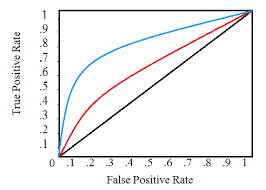
\includegraphics{images/roc_simple.png}

    The ROC curve plots the \textbf{true positive rate (sensitivity)}:

\[\frac{\text{true positives}}{\text{true positives} + \text{false negatives}}\]

versus the \textbf{false positive rate (1 - specificity)}:

\[\frac{\text{false positives}}{\text{true negatives} + \text{false positives}}\]

The true positives, false positives, true negatives, and false negatives
will have to be determined by hand because the ground truth is what we
as humans identify. To calculate the rates, we can construct a confusion
matrix which shows the number of actual values and number of predicted
values.

\begin{longtable}[]{@{}llll@{}}
\toprule
& Confusion Matrix & &\tabularnewline
\midrule
\endhead
& \textbf{Actual 1} & \textbf{Actual 0} &\tabularnewline
\textbf{Predicted 1} & True Postive & False Positive &\tabularnewline
\textbf{Predicted 0} & False Negative & True Negative &\tabularnewline
& & &\tabularnewline
\bottomrule
\end{longtable}

    \begin{Verbatim}[commandchars=\\\{\}]
{\color{incolor}In [{\color{incolor}1}]:} \PY{k+kn}{import} \PY{n+nn}{numpy} \PY{k}{as} \PY{n+nn}{np}
        
        \PY{k+kn}{import} \PY{n+nn}{matplotlib}\PY{n+nn}{.}\PY{n+nn}{pyplot} \PY{k}{as} \PY{n+nn}{plt}
        \PY{k+kn}{import} \PY{n+nn}{matplotlib}
        
        \PY{o}{\PYZpc{}}\PY{k}{matplotlib} inline
        
        
        \PY{k+kn}{from} \PY{n+nn}{detector} \PY{k}{import} \PY{n}{model}
\end{Verbatim}


    \hypertarget{construct-confusion-matrix}{%
\subsection{Construct Confusion
Matrix}\label{construct-confusion-matrix}}

    \begin{Verbatim}[commandchars=\\\{\}]
{\color{incolor}In [{\color{incolor}2}]:} \PY{n}{threshold\PYZus{}list} \PY{o}{=} \PY{p}{[}\PY{l+m+mf}{0.5}\PY{p}{,} \PY{l+m+mf}{0.6}\PY{p}{,} \PY{l+m+mf}{0.7}\PY{p}{,} \PY{l+m+mf}{0.8}\PY{p}{,} \PY{l+m+mf}{0.9}\PY{p}{,} \PY{l+m+mf}{0.99}\PY{p}{]}
        
        \PY{k}{for} \PY{n}{threshold} \PY{o+ow}{in} \PY{n}{threshold\PYZus{}list}\PY{p}{:}
            \PY{n}{model}\PY{p}{(}\PY{n}{image\PYZus{}path}\PY{o}{=}\PY{l+s+s1}{\PYZsq{}}\PY{l+s+s1}{images/target\PYZus{}tennis.jpg}\PY{l+s+s1}{\PYZsq{}}\PY{p}{,} \PY{n}{template\PYZus{}path}\PY{o}{=}\PY{l+s+s1}{\PYZsq{}}\PY{l+s+s1}{images/template\PYZus{}tennis.jpg}\PY{l+s+s1}{\PYZsq{}}\PY{p}{,}
                  \PY{n}{threshold}\PY{o}{=}\PY{n}{threshold}\PY{p}{,} \PY{n}{analyze}\PY{o}{=}\PY{k+kc}{True}\PY{p}{)}
\end{Verbatim}


    \begin{Verbatim}[commandchars=\\\{\}]
149 detections with threshold: 0.5


    \end{Verbatim}

    \begin{center}
    \adjustimage{max size={0.9\linewidth}{0.9\paperheight}}{output_5_1.png}
    \end{center}
    { \hspace*{\fill} \\}
    
    \begin{Verbatim}[commandchars=\\\{\}]
117 detections with threshold: 0.6


    \end{Verbatim}

    \begin{center}
    \adjustimage{max size={0.9\linewidth}{0.9\paperheight}}{output_5_3.png}
    \end{center}
    { \hspace*{\fill} \\}
    
    \begin{Verbatim}[commandchars=\\\{\}]
61 detections with threshold: 0.7


    \end{Verbatim}

    \begin{center}
    \adjustimage{max size={0.9\linewidth}{0.9\paperheight}}{output_5_5.png}
    \end{center}
    { \hspace*{\fill} \\}
    
    \begin{Verbatim}[commandchars=\\\{\}]
11 detections with threshold: 0.8


    \end{Verbatim}

    \begin{center}
    \adjustimage{max size={0.9\linewidth}{0.9\paperheight}}{output_5_7.png}
    \end{center}
    { \hspace*{\fill} \\}
    
    \begin{Verbatim}[commandchars=\\\{\}]
3 detections with threshold: 0.9


    \end{Verbatim}

    \begin{center}
    \adjustimage{max size={0.9\linewidth}{0.9\paperheight}}{output_5_9.png}
    \end{center}
    { \hspace*{\fill} \\}
    
    \begin{Verbatim}[commandchars=\\\{\}]
1 detections with threshold: 0.99


    \end{Verbatim}

    \begin{center}
    \adjustimage{max size={0.9\linewidth}{0.9\paperheight}}{output_5_11.png}
    \end{center}
    { \hspace*{\fill} \\}
    
    \hypertarget{ground-truth-values}{%
\subsubsection{Ground Truth Values}\label{ground-truth-values}}

The number of actual positives is easy: it is simply the number of
features in the image, in this example 9 tennis balls. A perfect model
would therefore identify all 9 tennis balls without classify any other
points as matches

Defining acutal negatives is difficult in this case. I will say that
actual negatives are every possible patch which does not contain the
feature. As the convolution calculates the response of every single
pixel, the number of possible patches is the pixel width times the pixel
height of the image. The number of actual negatives is therefore the
number of patches - the number of features in the image. For example,
our image is 162 * 312 and there are 9 occurences of the feature in the
image sothere are \((162 * 312) - 9 = 50535\) actual negatives in the
image. These actual negatives are locations where the model should
\emph{not} identify a feature. Defining the number of actual negatives
and the number of actual positives allows us to calculate the true
negatives and false positives.

    \begin{Verbatim}[commandchars=\\\{\}]
{\color{incolor}In [{\color{incolor}3}]:} \PY{n}{image} \PY{o}{=} \PY{n}{plt}\PY{o}{.}\PY{n}{imread}\PY{p}{(}\PY{l+s+s1}{\PYZsq{}}\PY{l+s+s1}{images/target\PYZus{}tennis.jpg}\PY{l+s+s1}{\PYZsq{}}\PY{p}{)}
        \PY{n}{actual\PYZus{}negatives} \PY{o}{=} \PY{p}{(}\PY{n}{image}\PY{o}{.}\PY{n}{shape}\PY{p}{[}\PY{l+m+mi}{0}\PY{p}{]} \PY{o}{*} \PY{n}{image}\PY{o}{.}\PY{n}{shape}\PY{p}{[}\PY{l+m+mi}{1}\PY{p}{]}\PY{p}{)} \PY{o}{\PYZhy{}} \PY{l+m+mi}{9}
        \PY{n+nb}{print}\PY{p}{(}\PY{l+s+s1}{\PYZsq{}}\PY{l+s+s1}{Number of actual negatives:}\PY{l+s+s1}{\PYZsq{}}\PY{p}{,} \PY{n}{actual\PYZus{}negatives}\PY{p}{)}
\end{Verbatim}


    \begin{Verbatim}[commandchars=\\\{\}]
Number of actual negatives: 50535

    \end{Verbatim}

    \hypertarget{first-list-of-results}{%
\subsubsection{First List of Results}\label{first-list-of-results}}

Following is the true positives, false positives, true negatives, and
false negatives for each of the thresholds. Using these numbers, we can
calculate the

\textbf{true positive rate}:

\[\frac{\text{true positives}}{\text{true positives} + \text{false negatives}}\]

for the y-axis

and the \textbf{false positive rate}:

\[\frac{\text{false positives}}{\text{true negatives} + \text{false positives}}\]

for the x-axis. This forms the ROC curve as a function of the threshold.

    \begin{Verbatim}[commandchars=\\\{\}]
{\color{incolor}In [{\color{incolor}19}]:} \PY{n}{threshold\PYZus{}list} \PY{o}{=} \PY{p}{[}\PY{l+m+mf}{0.5}\PY{p}{,} \PY{l+m+mf}{0.6}\PY{p}{,} \PY{l+m+mf}{0.7}\PY{p}{,} \PY{l+m+mf}{0.8}\PY{p}{,} \PY{l+m+mf}{0.9}\PY{p}{,} \PY{l+m+mf}{0.99}\PY{p}{]}
         
         \PY{n}{tp\PYZus{}list} \PY{o}{=} \PY{p}{[}\PY{l+m+mi}{9}\PY{p}{,} \PY{l+m+mi}{9}\PY{p}{,} \PY{l+m+mi}{9}\PY{p}{,} \PY{l+m+mi}{8}\PY{p}{,} \PY{l+m+mi}{3}\PY{p}{,} \PY{l+m+mi}{1}\PY{p}{]}
         \PY{n}{fp\PYZus{}list} \PY{o}{=} \PY{p}{[}\PY{l+m+mi}{140}\PY{p}{,} \PY{l+m+mi}{108}\PY{p}{,} \PY{l+m+mi}{52}\PY{p}{,} \PY{l+m+mi}{3}\PY{p}{,} \PY{l+m+mi}{0}\PY{p}{,} \PY{l+m+mi}{0}\PY{p}{]}
         \PY{n}{tn\PYZus{}list} \PY{o}{=} \PY{p}{[}\PY{l+m+mi}{50535} \PY{o}{\PYZhy{}} \PY{l+m+mi}{149}\PY{p}{,} \PY{l+m+mi}{50535} \PY{o}{\PYZhy{}} \PY{l+m+mi}{117}\PY{p}{,} \PY{l+m+mi}{50535} \PY{o}{\PYZhy{}} \PY{l+m+mi}{61}\PY{p}{,} 
                    \PY{l+m+mi}{50535} \PY{o}{\PYZhy{}} \PY{l+m+mi}{11}\PY{p}{,} \PY{l+m+mi}{50535} \PY{o}{\PYZhy{}} \PY{l+m+mi}{3}\PY{p}{,} \PY{l+m+mi}{50535} \PY{o}{\PYZhy{}} \PY{l+m+mi}{1}\PY{p}{]}
         \PY{n}{fn\PYZus{}list} \PY{o}{=} \PY{p}{[}\PY{l+m+mi}{0}\PY{p}{,} \PY{l+m+mi}{0}\PY{p}{,}  \PY{l+m+mi}{0}\PY{p}{,} \PY{l+m+mi}{1}\PY{p}{,} \PY{l+m+mi}{6}\PY{p}{,} \PY{l+m+mi}{10}\PY{p}{]}
\end{Verbatim}


    \hypertarget{function-to-plot-the-roc-curve}{%
\subsection{Function to Plot the ROC
Curve}\label{function-to-plot-the-roc-curve}}

    \begin{Verbatim}[commandchars=\\\{\}]
{\color{incolor}In [{\color{incolor}20}]:} \PY{k}{def} \PY{n+nf}{analyze\PYZus{}results}\PY{p}{(}\PY{n}{tp\PYZus{}list}\PY{p}{,} \PY{n}{fp\PYZus{}list}\PY{p}{,} \PY{n}{tn\PYZus{}list}\PY{p}{,} \PY{n}{fn\PYZus{}list}\PY{p}{,} \PY{n}{threshold\PYZus{}list}\PY{p}{,}
                            \PY{n}{actual\PYZus{}negatives}\PY{p}{,} \PY{n}{actual\PYZus{}positives}\PY{p}{)}\PY{p}{:}
             
             \PY{n}{tpr\PYZus{}list} \PY{o}{=} \PY{p}{[}\PY{p}{]}
             \PY{n}{fpr\PYZus{}list} \PY{o}{=} \PY{p}{[}\PY{p}{]}
             \PY{n}{plt}\PY{o}{.}\PY{n}{style}\PY{o}{.}\PY{n}{use}\PY{p}{(}\PY{l+s+s1}{\PYZsq{}}\PY{l+s+s1}{fivethirtyeight}\PY{l+s+s1}{\PYZsq{}}\PY{p}{)}
             \PY{n}{plt}\PY{o}{.}\PY{n}{figure}\PY{p}{(}\PY{n}{figsize}\PY{o}{=}\PY{p}{(}\PY{l+m+mi}{8}\PY{p}{,} \PY{l+m+mi}{8}\PY{p}{)}\PY{p}{)}
             \PY{n}{plt}\PY{o}{.}\PY{n}{xticks}\PY{p}{(}\PY{n}{rotation}\PY{o}{=}\PY{l+m+mi}{60}\PY{p}{)}
             
             \PY{k}{for} \PY{n}{tp}\PY{p}{,} \PY{n}{fp}\PY{p}{,} \PY{n}{tn}\PY{p}{,} \PY{n}{fn}\PY{p}{,} \PY{n}{threshold} \PY{o+ow}{in} \PY{n+nb}{zip}\PY{p}{(}\PY{n}{tp\PYZus{}list}\PY{p}{,} \PY{n}{fp\PYZus{}list}\PY{p}{,} 
                                                  \PY{n}{tn\PYZus{}list}\PY{p}{,} \PY{n}{fn\PYZus{}list}\PY{p}{,} 
                                                  \PY{n}{threshold\PYZus{}list}\PY{p}{)}\PY{p}{:}
                 
                 \PY{k}{if} \PY{n}{fp} \PY{o}{==} \PY{l+m+mi}{0}\PY{p}{:}
                     \PY{n}{fpr} \PY{o}{=} \PY{l+m+mi}{0}
                 \PY{k}{else}\PY{p}{:}
                     \PY{n}{fpr} \PY{o}{=} \PY{n}{fp} \PY{o}{/} \PY{p}{(}\PY{n}{fp} \PY{o}{+} \PY{n}{tn}\PY{p}{)}
         
                 \PY{n}{tpr} \PY{o}{=} \PY{n}{tp} \PY{o}{/} \PY{p}{(}\PY{n}{tp} \PY{o}{+} \PY{n}{fn}\PY{p}{)}
         
                 \PY{n}{tpr\PYZus{}list}\PY{o}{.}\PY{n}{append}\PY{p}{(}\PY{n}{tpr}\PY{p}{)}
                 \PY{n}{fpr\PYZus{}list}\PY{o}{.}\PY{n}{append}\PY{p}{(}\PY{n}{fpr}\PY{p}{)}
              
                 \PY{n}{plt}\PY{o}{.}\PY{n}{plot}\PY{p}{(}\PY{n}{fpr}\PY{p}{,} \PY{n}{tpr} \PY{o}{+} \PY{l+m+mf}{0.05}\PY{p}{,} \PY{n}{marker}\PY{o}{=}\PY{l+s+s1}{\PYZsq{}}\PY{l+s+s1}{\PYZdl{}}\PY{l+s+si}{\PYZpc{}.2f}\PY{l+s+s1}{\PYZdl{}}\PY{l+s+s1}{\PYZsq{}} \PY{o}{\PYZpc{}} \PY{n}{threshold}\PY{p}{,} 
                          \PY{n}{ms} \PY{o}{=} \PY{l+m+mi}{30}\PY{p}{,} \PY{n}{color} \PY{o}{=} \PY{l+s+s1}{\PYZsq{}}\PY{l+s+s1}{k}\PY{l+s+s1}{\PYZsq{}}\PY{p}{,} 
                         \PY{n}{label} \PY{o}{=} \PY{l+s+s1}{\PYZsq{}}\PY{l+s+s1}{threshold}\PY{l+s+s1}{\PYZsq{}}\PY{p}{)} 
                 
             \PY{n}{plt}\PY{o}{.}\PY{n}{plot}\PY{p}{(}\PY{n}{fpr\PYZus{}list}\PY{p}{,} \PY{n}{tpr\PYZus{}list}\PY{p}{,} \PY{l+s+s1}{\PYZsq{}}\PY{l+s+s1}{o\PYZhy{}}\PY{l+s+s1}{\PYZsq{}}\PY{p}{,} \PY{n}{color} \PY{o}{=} \PY{l+s+s1}{\PYZsq{}}\PY{l+s+s1}{red}\PY{l+s+s1}{\PYZsq{}}\PY{p}{)}\PY{p}{;} 
             \PY{n}{plt}\PY{o}{.}\PY{n}{xlabel}\PY{p}{(}\PY{l+s+s1}{\PYZsq{}}\PY{l+s+s1}{False Postive Rate}\PY{l+s+s1}{\PYZsq{}}\PY{p}{)}\PY{p}{;} \PY{n}{plt}\PY{o}{.}\PY{n}{ylabel}\PY{p}{(}\PY{l+s+s1}{\PYZsq{}}\PY{l+s+s1}{True Positive Rate}\PY{l+s+s1}{\PYZsq{}}\PY{p}{)}\PY{p}{;}
             \PY{n}{plt}\PY{o}{.}\PY{n}{title}\PY{p}{(}\PY{l+s+s1}{\PYZsq{}}\PY{l+s+s1}{ROC Curve}\PY{l+s+s1}{\PYZsq{}}\PY{p}{)}\PY{p}{;} 
             \PY{n}{plt}\PY{o}{.}\PY{n}{show}\PY{p}{(}\PY{p}{)}
\end{Verbatim}


    \begin{Verbatim}[commandchars=\\\{\}]
{\color{incolor}In [{\color{incolor}21}]:} \PY{n}{analyze\PYZus{}results}\PY{p}{(}\PY{n}{tp\PYZus{}list}\PY{p}{,} \PY{n}{fp\PYZus{}list}\PY{p}{,} \PY{n}{tn\PYZus{}list}\PY{p}{,} \PY{n}{fn\PYZus{}list}\PY{p}{,} \PY{n}{threshold\PYZus{}list}\PY{p}{,} 
                         \PY{n}{actual\PYZus{}negatives}\PY{o}{=}\PY{l+m+mi}{50535}\PY{p}{,} \PY{n}{actual\PYZus{}positives}\PY{o}{=}\PY{l+m+mi}{9}\PY{p}{)}
\end{Verbatim}


    \begin{center}
    \adjustimage{max size={0.9\linewidth}{0.9\paperheight}}{output_12_0.png}
    \end{center}
    { \hspace*{\fill} \\}
    
    \hypertarget{shifting-the-curve}{%
\subsection{Shifting the Curve}\label{shifting-the-curve}}

Altering the threshold shifts the location along one ROC curve. This
does not change the signal to noise ratio though, so this approach will
only move along the curve. To shift the curve requires changing the
signal to noise ratio.

One way to shift the curve would be to adjust how far apart boxes have
to be in the method, or using a different template. I will choose
another of the images for the template. Both of these approaches change
the signal to noise ratio. Changning the template image can increase or
decrease the signal depending on the quality of the template.

    \begin{Verbatim}[commandchars=\\\{\}]
{\color{incolor}In [{\color{incolor}7}]:} \PY{n}{threshold\PYZus{}list} \PY{o}{=} \PY{p}{[}\PY{l+m+mf}{0.5}\PY{p}{,} \PY{l+m+mf}{0.6}\PY{p}{,} \PY{l+m+mf}{0.7}\PY{p}{,} \PY{l+m+mf}{0.8}\PY{p}{,} \PY{l+m+mf}{0.9}\PY{p}{,} \PY{l+m+mf}{0.99}\PY{p}{]}
        
        \PY{k}{for} \PY{n}{threshold} \PY{o+ow}{in} \PY{n}{threshold\PYZus{}list}\PY{p}{:}
            \PY{n}{model}\PY{p}{(}\PY{n}{image\PYZus{}path}\PY{o}{=}\PY{l+s+s1}{\PYZsq{}}\PY{l+s+s1}{images/target\PYZus{}tennis.jpg}\PY{l+s+s1}{\PYZsq{}}\PY{p}{,} 
                  \PY{n}{template\PYZus{}path}\PY{o}{=}\PY{l+s+s1}{\PYZsq{}}\PY{l+s+s1}{images/template\PYZus{}tennis\PYZus{}two.jpg}\PY{l+s+s1}{\PYZsq{}}\PY{p}{,}
                  \PY{n}{threshold}\PY{o}{=}\PY{n}{threshold}\PY{p}{,} \PY{n}{analyze}\PY{o}{=}\PY{k+kc}{True}\PY{p}{)}
\end{Verbatim}


    \begin{Verbatim}[commandchars=\\\{\}]
133 detections with threshold: 0.5


    \end{Verbatim}

    \begin{center}
    \adjustimage{max size={0.9\linewidth}{0.9\paperheight}}{output_14_1.png}
    \end{center}
    { \hspace*{\fill} \\}
    
    \begin{Verbatim}[commandchars=\\\{\}]
102 detections with threshold: 0.6


    \end{Verbatim}

    \begin{center}
    \adjustimage{max size={0.9\linewidth}{0.9\paperheight}}{output_14_3.png}
    \end{center}
    { \hspace*{\fill} \\}
    
    \begin{Verbatim}[commandchars=\\\{\}]
45 detections with threshold: 0.7


    \end{Verbatim}

    \begin{center}
    \adjustimage{max size={0.9\linewidth}{0.9\paperheight}}{output_14_5.png}
    \end{center}
    { \hspace*{\fill} \\}
    
    \begin{Verbatim}[commandchars=\\\{\}]
7 detections with threshold: 0.8


    \end{Verbatim}

    \begin{center}
    \adjustimage{max size={0.9\linewidth}{0.9\paperheight}}{output_14_7.png}
    \end{center}
    { \hspace*{\fill} \\}
    
    \begin{Verbatim}[commandchars=\\\{\}]
2 detections with threshold: 0.9


    \end{Verbatim}

    \begin{center}
    \adjustimage{max size={0.9\linewidth}{0.9\paperheight}}{output_14_9.png}
    \end{center}
    { \hspace*{\fill} \\}
    
    \begin{Verbatim}[commandchars=\\\{\}]
1 detections with threshold: 0.99


    \end{Verbatim}

    \begin{center}
    \adjustimage{max size={0.9\linewidth}{0.9\paperheight}}{output_14_11.png}
    \end{center}
    { \hspace*{\fill} \\}
    
    \begin{Verbatim}[commandchars=\\\{\}]
{\color{incolor}In [{\color{incolor}23}]:} \PY{n}{tp\PYZus{}list} \PY{o}{=} \PY{p}{[}\PY{l+m+mi}{9}\PY{p}{,} \PY{l+m+mi}{9}\PY{p}{,} \PY{l+m+mi}{9}\PY{p}{,} \PY{l+m+mi}{6}\PY{p}{,} \PY{l+m+mi}{2}\PY{p}{,} \PY{l+m+mi}{1}\PY{p}{]}
         \PY{n}{fp\PYZus{}list} \PY{o}{=} \PY{p}{[}\PY{l+m+mi}{124}\PY{p}{,} \PY{l+m+mi}{93}\PY{p}{,} \PY{l+m+mi}{36}\PY{p}{,} \PY{l+m+mi}{1}\PY{p}{,} \PY{l+m+mi}{0}\PY{p}{,} \PY{l+m+mi}{0}\PY{p}{]}
         \PY{n}{tn\PYZus{}list} \PY{o}{=} \PY{p}{[}\PY{l+m+mi}{50535} \PY{o}{\PYZhy{}} \PY{l+m+mi}{133}\PY{p}{,} \PY{l+m+mi}{50535} \PY{o}{\PYZhy{}} \PY{l+m+mi}{102}\PY{p}{,} \PY{l+m+mi}{50535} \PY{o}{\PYZhy{}} \PY{l+m+mi}{45}\PY{p}{,} 
                    \PY{l+m+mi}{50535} \PY{o}{\PYZhy{}} \PY{l+m+mi}{7}\PY{p}{,} \PY{l+m+mi}{50535} \PY{o}{\PYZhy{}} \PY{l+m+mi}{2}\PY{p}{,} \PY{l+m+mi}{50535} \PY{o}{\PYZhy{}} \PY{l+m+mi}{1}\PY{p}{]}
         \PY{n}{fn\PYZus{}list} \PY{o}{=} \PY{p}{[}\PY{l+m+mi}{0}\PY{p}{,} \PY{l+m+mi}{0}\PY{p}{,}  \PY{l+m+mi}{0}\PY{p}{,} \PY{l+m+mi}{3}\PY{p}{,} \PY{l+m+mi}{9}\PY{p}{,} \PY{l+m+mi}{10}\PY{p}{]}
\end{Verbatim}


    \begin{Verbatim}[commandchars=\\\{\}]
{\color{incolor}In [{\color{incolor}24}]:} \PY{n}{analyze\PYZus{}results}\PY{p}{(}\PY{n}{tp\PYZus{}list}\PY{p}{,} \PY{n}{fp\PYZus{}list}\PY{p}{,} \PY{n}{tn\PYZus{}list}\PY{p}{,} \PY{n}{fn\PYZus{}list}\PY{p}{,}
                         \PY{n}{threshold\PYZus{}list}\PY{p}{,} \PY{n}{actual\PYZus{}negatives}\PY{o}{=}\PY{l+m+mi}{50535}\PY{p}{,} \PY{n}{actual\PYZus{}positives}\PY{o}{=}\PY{l+m+mi}{9}\PY{p}{)}
\end{Verbatim}


    \begin{center}
    \adjustimage{max size={0.9\linewidth}{0.9\paperheight}}{output_16_0.png}
    \end{center}
    { \hspace*{\fill} \\}
    
    \hypertarget{blur-the-image-before-detecting-features}{%
\subsection{Blur the Image before Detecting
Features}\label{blur-the-image-before-detecting-features}}

    Another approach to shift the curve is to blur the image using a
Gaussian kernel before detecting images. The Gaussian blur decreases the
amount of noise in the image, so we would expect the ROC curve to shift
up and to the left with the pre-processing step.

    \begin{Verbatim}[commandchars=\\\{\}]
{\color{incolor}In [{\color{incolor}15}]:} \PY{k+kn}{from} \PY{n+nn}{PIL} \PY{k}{import} \PY{n}{Image}
         \PY{k+kn}{import} \PY{n+nn}{matplotlib} \PY{k}{as} \PY{n+nn}{mpl}
         
         \PY{k}{def} \PY{n+nf}{apply\PYZus{}blur\PYZus{}filter}\PY{p}{(}\PY{n}{blur\PYZus{}filter}\PY{p}{,} \PY{n}{image\PYZus{}path}\PY{p}{)}\PY{p}{:}
             
             \PY{c+c1}{\PYZsh{} Load in the image}
             \PY{n}{image} \PY{o}{=} \PY{n}{Image}\PY{o}{.}\PY{n}{open}\PY{p}{(}\PY{n}{image\PYZus{}path}\PY{p}{)}
             
             \PY{c+c1}{\PYZsh{} Crop to correct size}
             \PY{n}{image} \PY{o}{=} \PY{n}{image}\PY{o}{.}\PY{n}{crop}\PY{p}{(}\PY{n}{box}\PY{o}{=}\PY{p}{(}\PY{l+m+mi}{0}\PY{p}{,} \PY{l+m+mi}{0}\PY{p}{,} 
                                \PY{n+nb}{int}\PY{p}{(}\PY{n}{image}\PY{o}{.}\PY{n}{size}\PY{p}{[}\PY{l+m+mi}{0}\PY{p}{]} \PY{o}{/} \PY{n}{blur\PYZus{}filter}\PY{o}{.}\PY{n}{shape}\PY{p}{[}\PY{l+m+mi}{0}\PY{p}{]}\PY{p}{)} \PY{o}{*} \PY{n}{blur\PYZus{}filter}\PY{o}{.}\PY{n}{shape}\PY{p}{[}\PY{l+m+mi}{0}\PY{p}{]}\PY{p}{,} 
                                \PY{n+nb}{int}\PY{p}{(}\PY{n}{image}\PY{o}{.}\PY{n}{size}\PY{p}{[}\PY{l+m+mi}{1}\PY{p}{]} \PY{o}{/} \PY{n}{blur\PYZus{}filter}\PY{o}{.}\PY{n}{shape}\PY{p}{[}\PY{l+m+mi}{1}\PY{p}{]}\PY{p}{)} \PY{o}{*} \PY{n}{blur\PYZus{}filter}\PY{o}{.}\PY{n}{shape}\PY{p}{[}\PY{l+m+mi}{1}\PY{p}{]}\PY{p}{)}\PY{p}{)}
             
             \PY{n}{im\PYZus{}array} \PY{o}{=} \PY{n}{np}\PY{o}{.}\PY{n}{array}\PY{p}{(}\PY{n}{image}\PY{p}{)}
             
             \PY{c+c1}{\PYZsh{} Horizontal and vertical moves, using a stride of filter shape}
             \PY{n}{h\PYZus{}moves} \PY{o}{=} \PY{n+nb}{int}\PY{p}{(}\PY{n}{im\PYZus{}array}\PY{o}{.}\PY{n}{shape}\PY{p}{[}\PY{l+m+mi}{1}\PY{p}{]} \PY{o}{/} \PY{n}{blur\PYZus{}filter}\PY{o}{.}\PY{n}{shape}\PY{p}{[}\PY{l+m+mi}{1}\PY{p}{]}\PY{p}{)}
             \PY{n}{v\PYZus{}moves} \PY{o}{=} \PY{n+nb}{int}\PY{p}{(}\PY{n}{im\PYZus{}array}\PY{o}{.}\PY{n}{shape}\PY{p}{[}\PY{l+m+mi}{0}\PY{p}{]} \PY{o}{/} \PY{n}{blur\PYZus{}filter}\PY{o}{.}\PY{n}{shape}\PY{p}{[}\PY{l+m+mi}{0}\PY{p}{]}\PY{p}{)}
             
             \PY{n}{new\PYZus{}image} \PY{o}{=} \PY{n}{np}\PY{o}{.}\PY{n}{zeros}\PY{p}{(}\PY{n}{shape} \PY{o}{=} \PY{n}{im\PYZus{}array}\PY{o}{.}\PY{n}{shape}\PY{p}{)}
             
             \PY{n}{k} \PY{o}{=} \PY{n}{np}\PY{o}{.}\PY{n}{sum}\PY{p}{(}\PY{n}{blur\PYZus{}filter}\PY{p}{)}
             
             \PY{c+c1}{\PYZsh{} Iterate through 3 color channels}
             \PY{k}{for} \PY{n}{i} \PY{o+ow}{in} \PY{n+nb}{range}\PY{p}{(}\PY{n}{im\PYZus{}array}\PY{o}{.}\PY{n}{shape}\PY{p}{[}\PY{l+m+mi}{2}\PY{p}{]}\PY{p}{)}\PY{p}{:}
                 \PY{c+c1}{\PYZsh{} Extract the layer and create a new layer to fill in }
                 \PY{n}{layer} \PY{o}{=} \PY{n}{im\PYZus{}array}\PY{p}{[}\PY{p}{:}\PY{p}{,} \PY{p}{:}\PY{p}{,} \PY{n}{i}\PY{p}{]}
                 \PY{n}{new\PYZus{}layer} \PY{o}{=} \PY{n}{np}\PY{o}{.}\PY{n}{zeros}\PY{p}{(}\PY{n}{shape} \PY{o}{=} \PY{n}{layer}\PY{o}{.}\PY{n}{shape}\PY{p}{,} \PY{n}{dtype}\PY{o}{=}\PY{l+s+s1}{\PYZsq{}}\PY{l+s+s1}{uint8}\PY{l+s+s1}{\PYZsq{}}\PY{p}{)}
         
                 \PY{c+c1}{\PYZsh{} Left and right bounds are determined by columns}
                 \PY{n}{l\PYZus{}border} \PY{o}{=} \PY{l+m+mi}{0}
                 \PY{n}{r\PYZus{}border} \PY{o}{=} \PY{n}{blur\PYZus{}filter}\PY{o}{.}\PY{n}{shape}\PY{p}{[}\PY{l+m+mi}{1}\PY{p}{]}
         
         
                 \PY{c+c1}{\PYZsh{} Iterate through the number of horizontal and vertical moves}
                 \PY{k}{for} \PY{n}{h} \PY{o+ow}{in} \PY{n+nb}{range}\PY{p}{(}\PY{n}{h\PYZus{}moves}\PY{p}{)}\PY{p}{:}
                     \PY{c+c1}{\PYZsh{} Top and bottom bounds are determined by rows}
                     \PY{n}{b\PYZus{}border} \PY{o}{=} \PY{l+m+mi}{0}
                     \PY{n}{t\PYZus{}border} \PY{o}{=} \PY{n}{blur\PYZus{}filter}\PY{o}{.}\PY{n}{shape}\PY{p}{[}\PY{l+m+mi}{0}\PY{p}{]}
                     \PY{k}{for} \PY{n}{v} \PY{o+ow}{in} \PY{n+nb}{range}\PY{p}{(}\PY{n}{v\PYZus{}moves}\PY{p}{)}\PY{p}{:}
                         \PY{n}{patch} \PY{o}{=} \PY{n}{layer}\PY{p}{[}\PY{n}{b\PYZus{}border}\PY{p}{:}\PY{n}{t\PYZus{}border}\PY{p}{,} \PY{n}{l\PYZus{}border}\PY{p}{:}\PY{n}{r\PYZus{}border}\PY{p}{]}
         
                         \PY{c+c1}{\PYZsh{} Take the element\PYZhy{}wise product of the patch and the filter}
                         \PY{n}{product} \PY{o}{=} \PY{n}{np}\PY{o}{.}\PY{n}{multiply}\PY{p}{(}\PY{n}{patch}\PY{p}{,} \PY{n}{blur\PYZus{}filter}\PY{p}{)}
         
                         \PY{c+c1}{\PYZsh{} Find the weighted average of the patch}
                         \PY{n}{product} \PY{o}{=} \PY{n}{np}\PY{o}{.}\PY{n}{sum}\PY{p}{(}\PY{n}{product}\PY{p}{)} \PY{o}{/} \PY{n}{k}
                         \PY{n}{new\PYZus{}layer}\PY{p}{[}\PY{n}{b\PYZus{}border}\PY{p}{:}\PY{n}{t\PYZus{}border}\PY{p}{,} \PY{n}{l\PYZus{}border}\PY{p}{:}\PY{n}{r\PYZus{}border}\PY{p}{]} \PY{o}{=} \PY{n}{product}
         
                         \PY{n}{b\PYZus{}border} \PY{o}{=} \PY{n}{t\PYZus{}border}
                         \PY{n}{t\PYZus{}border} \PY{o}{=} \PY{n}{t\PYZus{}border} \PY{o}{+} \PY{n}{blur\PYZus{}filter}\PY{o}{.}\PY{n}{shape}\PY{p}{[}\PY{l+m+mi}{0}\PY{p}{]}
         
                     \PY{n}{l\PYZus{}border} \PY{o}{=} \PY{n}{r\PYZus{}border}
                     \PY{n}{r\PYZus{}border} \PY{o}{=} \PY{n}{r\PYZus{}border} \PY{o}{+} \PY{n}{blur\PYZus{}filter}\PY{o}{.}\PY{n}{shape}\PY{p}{[}\PY{l+m+mi}{1}\PY{p}{]}
         
         
                 \PY{n}{new\PYZus{}image}\PY{p}{[}\PY{p}{:}\PY{p}{,} \PY{p}{:}\PY{p}{,} \PY{n}{i}\PY{p}{]} \PY{o}{=} \PY{l+m+mi}{255} \PY{o}{*} \PY{p}{(} \PY{p}{(}\PY{n}{new\PYZus{}layer} \PY{o}{\PYZhy{}} \PY{n}{np}\PY{o}{.}\PY{n}{min}\PY{p}{(}\PY{n}{new\PYZus{}layer}\PY{p}{)}\PY{p}{)} \PY{o}{/} 
                                             \PY{p}{(}\PY{n}{np}\PY{o}{.}\PY{n}{max}\PY{p}{(}\PY{n}{new\PYZus{}layer}\PY{p}{)} \PY{o}{\PYZhy{}} \PY{n}{np}\PY{o}{.}\PY{n}{min}\PY{p}{(}\PY{n}{new\PYZus{}layer}\PY{p}{)}\PY{p}{)} \PY{p}{)}
         
         
             \PY{c+c1}{\PYZsh{} Convert to correct type for plotting}
             \PY{n}{new\PYZus{}image} \PY{o}{=} \PY{n}{new\PYZus{}image}\PY{o}{.}\PY{n}{astype}\PY{p}{(}\PY{l+s+s1}{\PYZsq{}}\PY{l+s+s1}{uint8}\PY{l+s+s1}{\PYZsq{}}\PY{p}{)}
             
             \PY{k}{return} \PY{n}{new\PYZus{}image}
         
         \PY{n}{gaussian\PYZus{}kernel} \PY{o}{=} \PY{n}{np}\PY{o}{.}\PY{n}{array}\PY{p}{(}\PY{p}{[}\PY{p}{[}\PY{l+m+mi}{1}\PY{p}{,} \PY{l+m+mi}{4}\PY{p}{,} \PY{l+m+mi}{6}\PY{p}{,} \PY{l+m+mi}{4}\PY{p}{,} \PY{l+m+mi}{1}\PY{p}{]}\PY{p}{,}
                                     \PY{p}{[}\PY{l+m+mi}{2}\PY{p}{,} \PY{l+m+mi}{8}\PY{p}{,} \PY{l+m+mi}{12}\PY{p}{,} \PY{l+m+mi}{8}\PY{p}{,} \PY{l+m+mi}{2}\PY{p}{]}\PY{p}{,}
                                     \PY{p}{[}\PY{l+m+mi}{6}\PY{p}{,} \PY{l+m+mi}{24}\PY{p}{,} \PY{l+m+mi}{36}\PY{p}{,} \PY{l+m+mi}{24}\PY{p}{,} \PY{l+m+mi}{6}\PY{p}{]}\PY{p}{,}
                                     \PY{p}{[}\PY{l+m+mi}{2}\PY{p}{,} \PY{l+m+mi}{8}\PY{p}{,} \PY{l+m+mi}{12}\PY{p}{,} \PY{l+m+mi}{8}\PY{p}{,} \PY{l+m+mi}{2}\PY{p}{]}\PY{p}{,}
                                     \PY{p}{[}\PY{l+m+mi}{1}\PY{p}{,} \PY{l+m+mi}{4}\PY{p}{,} \PY{l+m+mi}{6}\PY{p}{,} \PY{l+m+mi}{4}\PY{p}{,} \PY{l+m+mi}{1}\PY{p}{]}\PY{p}{]}\PY{p}{)}
         
         \PY{n}{blur\PYZus{}tennis} \PY{o}{=} \PY{n}{apply\PYZus{}blur\PYZus{}filter}\PY{p}{(}\PY{n}{gaussian\PYZus{}kernel}\PY{p}{,} \PY{l+s+s1}{\PYZsq{}}\PY{l+s+s1}{images/target\PYZus{}tennis.jpg}\PY{l+s+s1}{\PYZsq{}}\PY{p}{)}
         \PY{n}{mpl}\PY{o}{.}\PY{n}{image}\PY{o}{.}\PY{n}{imsave}\PY{p}{(}\PY{l+s+s1}{\PYZsq{}}\PY{l+s+s1}{images/target\PYZus{}tennis\PYZus{}blurred.jpg}\PY{l+s+s1}{\PYZsq{}}\PY{p}{,} \PY{n}{blur\PYZus{}tennis}\PY{p}{)}
\end{Verbatim}


    \begin{Verbatim}[commandchars=\\\{\}]
{\color{incolor}In [{\color{incolor}16}]:} \PY{n}{threshold\PYZus{}list} \PY{o}{=} \PY{p}{[}\PY{l+m+mf}{0.5}\PY{p}{,} \PY{l+m+mf}{0.6}\PY{p}{,} \PY{l+m+mf}{0.7}\PY{p}{,} \PY{l+m+mf}{0.8}\PY{p}{,} \PY{l+m+mf}{0.9}\PY{p}{,} \PY{l+m+mf}{0.99}\PY{p}{]}
         
         \PY{k}{for} \PY{n}{threshold} \PY{o+ow}{in} \PY{n}{threshold\PYZus{}list}\PY{p}{:}
             \PY{n}{model}\PY{p}{(}\PY{n}{image\PYZus{}path}\PY{o}{=}\PY{l+s+s1}{\PYZsq{}}\PY{l+s+s1}{images/target\PYZus{}tennis\PYZus{}blurred.jpg}\PY{l+s+s1}{\PYZsq{}}\PY{p}{,} 
                   \PY{n}{template\PYZus{}path}\PY{o}{=}\PY{l+s+s1}{\PYZsq{}}\PY{l+s+s1}{images/template\PYZus{}tennis.jpg}\PY{l+s+s1}{\PYZsq{}}\PY{p}{,}
                   \PY{n}{threshold}\PY{o}{=}\PY{n}{threshold}\PY{p}{,} \PY{n}{analyze}\PY{o}{=}\PY{k+kc}{True}\PY{p}{)}
\end{Verbatim}


    \begin{Verbatim}[commandchars=\\\{\}]
59 detections with threshold: 0.5


    \end{Verbatim}

    \begin{center}
    \adjustimage{max size={0.9\linewidth}{0.9\paperheight}}{output_20_1.png}
    \end{center}
    { \hspace*{\fill} \\}
    
    \begin{Verbatim}[commandchars=\\\{\}]
14 detections with threshold: 0.6


    \end{Verbatim}

    \begin{center}
    \adjustimage{max size={0.9\linewidth}{0.9\paperheight}}{output_20_3.png}
    \end{center}
    { \hspace*{\fill} \\}
    
    \begin{Verbatim}[commandchars=\\\{\}]
9 detections with threshold: 0.7


    \end{Verbatim}

    \begin{center}
    \adjustimage{max size={0.9\linewidth}{0.9\paperheight}}{output_20_5.png}
    \end{center}
    { \hspace*{\fill} \\}
    
    \begin{Verbatim}[commandchars=\\\{\}]
5 detections with threshold: 0.8


    \end{Verbatim}

    \begin{center}
    \adjustimage{max size={0.9\linewidth}{0.9\paperheight}}{output_20_7.png}
    \end{center}
    { \hspace*{\fill} \\}
    
    \begin{Verbatim}[commandchars=\\\{\}]
1 detections with threshold: 0.9


    \end{Verbatim}

    \begin{center}
    \adjustimage{max size={0.9\linewidth}{0.9\paperheight}}{output_20_9.png}
    \end{center}
    { \hspace*{\fill} \\}
    
    \begin{Verbatim}[commandchars=\\\{\}]
0 detections with threshold: 0.99


    \end{Verbatim}

    \begin{center}
    \adjustimage{max size={0.9\linewidth}{0.9\paperheight}}{output_20_11.png}
    \end{center}
    { \hspace*{\fill} \\}
    
    \begin{Verbatim}[commandchars=\\\{\}]
{\color{incolor}In [{\color{incolor}25}]:} \PY{n}{threshold\PYZus{}list} \PY{o}{=} \PY{p}{[}\PY{l+m+mf}{0.5}\PY{p}{,} \PY{l+m+mf}{0.6}\PY{p}{,} \PY{l+m+mf}{0.7}\PY{p}{,} \PY{l+m+mf}{0.8}\PY{p}{,} \PY{l+m+mf}{0.9}\PY{p}{,} \PY{l+m+mf}{0.99}\PY{p}{]}
         
         \PY{n}{tp\PYZus{}list} \PY{o}{=} \PY{p}{[}\PY{l+m+mi}{9}\PY{p}{,} \PY{l+m+mi}{9}\PY{p}{,} \PY{l+m+mi}{9}\PY{p}{,} \PY{l+m+mi}{5}\PY{p}{,} \PY{l+m+mi}{1}\PY{p}{,} \PY{l+m+mi}{0}\PY{p}{]}
         \PY{n}{fp\PYZus{}list} \PY{o}{=} \PY{p}{[}\PY{l+m+mi}{50}\PY{p}{,} \PY{l+m+mi}{5}\PY{p}{,} \PY{l+m+mi}{0}\PY{p}{,} \PY{l+m+mi}{0}\PY{p}{,} \PY{l+m+mi}{0}\PY{p}{,} \PY{l+m+mi}{0}\PY{p}{]}
         \PY{n}{tn\PYZus{}list} \PY{o}{=} \PY{p}{[}\PY{l+m+mi}{50535} \PY{o}{\PYZhy{}} \PY{l+m+mi}{59}\PY{p}{,} \PY{l+m+mi}{50535} \PY{o}{\PYZhy{}} \PY{l+m+mi}{14}\PY{p}{,} \PY{l+m+mi}{50535} \PY{o}{\PYZhy{}} \PY{l+m+mi}{9}\PY{p}{,} 
                    \PY{l+m+mi}{50535} \PY{o}{\PYZhy{}} \PY{l+m+mi}{5}\PY{p}{,} \PY{l+m+mi}{50535} \PY{o}{\PYZhy{}} \PY{l+m+mi}{1}\PY{p}{,} \PY{l+m+mi}{50535}\PY{p}{]}
         \PY{n}{fn\PYZus{}list} \PY{o}{=} \PY{p}{[}\PY{l+m+mi}{0}\PY{p}{,} \PY{l+m+mi}{0}\PY{p}{,} \PY{l+m+mi}{0}\PY{p}{,} \PY{l+m+mi}{3}\PY{p}{,} \PY{l+m+mi}{8}\PY{p}{,} \PY{l+m+mi}{9}\PY{p}{]}
\end{Verbatim}


    \begin{Verbatim}[commandchars=\\\{\}]
{\color{incolor}In [{\color{incolor}26}]:} \PY{n}{analyze\PYZus{}results}\PY{p}{(}\PY{n}{tp\PYZus{}list}\PY{p}{,} \PY{n}{fp\PYZus{}list}\PY{p}{,} \PY{n}{tn\PYZus{}list}\PY{p}{,} \PY{n}{fn\PYZus{}list}\PY{p}{,}
                         \PY{n}{threshold\PYZus{}list}\PY{p}{,} \PY{n}{actual\PYZus{}negatives}\PY{o}{=}\PY{l+m+mi}{50535}\PY{p}{,} \PY{n}{actual\PYZus{}positives}\PY{o}{=}\PY{l+m+mi}{9}\PY{p}{)}
\end{Verbatim}


    \begin{center}
    \adjustimage{max size={0.9\linewidth}{0.9\paperheight}}{output_22_0.png}
    \end{center}
    { \hspace*{\fill} \\}
    
    Smoothing the image with a Gaussian Blur before feature detection and
using a threshold of 0.7 results in a perfect classifier! The signal to
noise ratio is changed by altering the content of the target image. This
shows the benefits or pre-processing images using methods such as
\href{https://homepages.inf.ed.ac.uk/rbf/HIPR2/gsmooth.htm}{Gaussian
Smoothing} before perform image analysis.

    \hypertarget{conclusions}{%
\section{Conclusions}\label{conclusions}}

In this notebook we created the Receiver Operating Characteristic Curve
for the feature detection model. The ROC curve plots the true positive
rate versus the false positive rate with a perfect classifier achieving
a tpr of 1.0 and a fpr of 0.0. We can change the location along a given
ROC curve be adjusting the threshold for establishing a detection based
on the convolution results. However, to shift the entire curve requires
changing the signal to noise ratio. We can do this by using a different
template, in this case a different image of the object we want to find.
Another approach that works well (in this case making a perfect
classifier) is applying pre-processing, such as a Gaussian Blur, to
smooth the image. Smoothing the image with a Gaussian filter removes
noise and details from the image resulting in fewer false positives.
This notebook showed the idea of using the ROC to assess model
performance, how to more along a given ROC curve, and using
pre-processing to shift the entire curve.


    % Add a bibliography block to the postdoc
    
    
    
    \end{document}
